\documentclass[12pt]{article}
\usepackage{amsmath}
\usepackage{tikz}
\begin{document}
\title{Statistics 12, Homework 4}
\date{February 17th, 2019}
\author{Michael Wu\\UID: 404751542}
\maketitle

\section*{Chapter 14, Problem 2}

Let \(A\) be ``likes to cook'' and \(B\) be ``likes to shop''. Then we have the following.
\[P(A)\cup P(B) = P(A) + P(B) - P(A\cap B)=0.45 + 0.59 - 0.23=0.81\]

\section*{Chapter 14, Problem 4}

\[\frac{38}{38+22}\approx0.633\]

\section*{Chapter 14, Problem 6}

\[0.7\times0.9=0.63\]

\section*{Chapter 14, Problem 10}

\begin{center}
    \begin{tabular}{c|cc|c}
        & Bank Online & Does Not Bank Online & Total\\
        \hline
        Younger than 50 & 0.25 & 0.15 & 0.4\\
        Not Younger than 50 & 0.05 & 0.55 & 0.6\\
        \hline
        Total & 0.3 & 0.7 & 1
    \end{tabular}
\end{center}
A table is better than a tree here because it requires less calculation to use. Instead of having
to multiply probabilities to arrive at the given percentages, the table presents the data
in the same way that it's given to us.

\section*{Chapter 14, Problem 12}

\begin{center}
    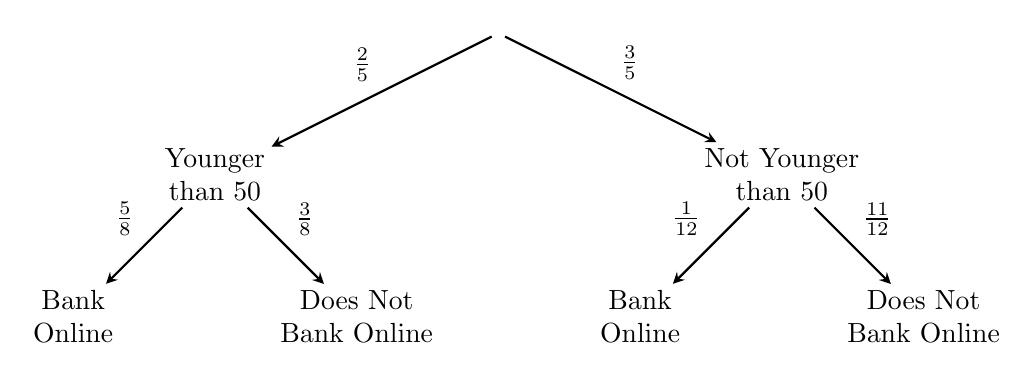
\begin{tikzpicture}[scale=0.9]
        \begin{scope}[auto, every node/.style={thick,rectangle,minimum size=0em,inner sep=2, align=center}]
            \node (Root) at (0,0) {};
            \node (Lt50) at (-4,-2) {Younger\\than 50};
            \node (Gt50) at (4,-2) {Not Younger\\than 50};
            \node (Online1) at (-6,-4) {Bank\\Online};
            \node (NotOnline1) at (-2,-4) {Does Not\\Bank Online};
            \node (Online2) at (2,-4) {Bank\\Online};
            \node (NotOnline2) at (6,-4) {Does Not\\Bank Online};
        \end{scope}
        \begin{scope}[auto, every node/.style={minimum size=0em}, every path/.style={thick, ->, >=stealth}]
            \path (Root) edge [above left] node {\(\frac{2}{5}\)} (Lt50);
            \path (Root) edge [above right] node {\(\frac{3}{5}\)}(Gt50);
            \path (Lt50) edge [above left] node {\(\frac{5}{8}\)} (Online1);
            \path (Lt50) edge [above right] node {\(\frac{3}{8}\)}(NotOnline1);
            \path (Gt50) edge [above left] node {\(\frac{1}{12}\)}(Online2);
            \path (Gt50) edge [above right] node {\(\frac{11}{12}\)}(NotOnline2);
        \end{scope}
    \end{tikzpicture}
\end{center}
A tree is better than a table in this case because we are given conditional probabilities. So it is easier
to express the probabilities in a way that matches the given data using a tree. The joint probabilities are
found by multiplying the conditional probabilities as you travel down a path in the tree.

\section*{Chapter 14, Problem 14}

\[\frac{\frac{2}{5}\times\frac{5}{8}}{\frac{2}{5}\times\frac{5}{8}+\frac{3}{5}\times\frac{1}{12}}\approx0.8333\]

\section*{Chapter 15, Problem 6}

\section*{Chapter 15, Problem 8}

\section*{Chapter 15, Problem 12}

\section*{Chapter 16, Problem 4}

\section*{Chapter 16, Problem 6}

\section*{Chapter 16, Problem 28}

\end{document}